\section{Qualitätssicherung}\label{quality-assurance}

Die grossen Datenmengen in diesem Projekt verlangten einen methodischen Ansatz zum Validieren der Qualität,
da eine Überprüfung aller Resultate aufgrund der grossen Anzahl und der Zeiteinschränkung nicht machbar war.
Aufgrund des zeitlichen Rahmens war eine systematische Bewertung der Qualität der Ergebnisse
nur bei der Extraktion der Zitate machbar.
Um ein ganzheitlicheres Bild über die Qualität der Auswertung erhalten zu können,
müssten die anderen Teile auch systematisch getestet und bewertet werden.

Die Qualität der Funktionen zum Erkennen der Zitate und Bestimmen des Geschlechts wurden ebenfalls mithilfe von
Gradings sichergestellt. Diese waren besonders während dem Entwickeln relevant und wurden deshalb aus praktischen Gründen
nicht weiter verfeinert. Die Algorithmen funktionieren mit zufriedenstellender Qualität, gemessen an Stichproben,
die wir von Hand durchgeführt haben.

Weil die Extraktion der Zitate im Gegensatz dazu keiner eindeutigen Logik folgen kann, war es für die Entwicklung dieses Algorithmus
wichtig, die Qualität und die Verbesserung des Algorithmus zu messen. Dies ermöglicht es uns ausserdem die Qualität
der Resultate abzuschätzen. 
Ein eigens dafür entwickelter Bewertungsalgorithmus soll einen möglichst guten Überblick über die Anzahl
der gefundenen Zitate und deren Qualität geben.

Dazu haben wir in manueller Arbeit pro Nachrichtenportal fünf Artikel ausgewertet und als JSON abgelegt. Insgesamt ergeben
sich daraus 20 Test-Artikel. Der Bewertungsalgorithmus ruft die Funktionalität zum Extrahieren der Zitate mit dem rohen
Text der Artikel auf und vergleicht das Resultat im Anschluss mit den manuell erstellten Lösungen. Als wichtigste Metrik
dient dabei der \enquote{Recall} (Abbildung \ref{recall-formula}).

\subsection{Recall}

Diese Metrik wird häufig auch im \gl{ml} verwendet, um die Genauigkeit des trainierten
Modells zu messen. Der Recall sagt in unserem Fall aus, wie viele der relevanten Zitate der Algorithmus finden konnte.
Der Recall ist die Prozentzahl der totalen Anzahl Zitate, die er hätte finden können.

\begin{figure}[H]
    \begin{equation}
        Recall = \frac{Anzahl \, gefundene \, Zitate}{Totale \, Anzahl \, Zitate}
    \end{equation}
    \caption{Formel Recall}
    \label{recall-formula}
\end{figure}

Als gefundene Zitate zählt der Bewertungsalgorithmus all diejenigen Zitate, die eine Qualität von
mindestens 60\% aufweisen. Mehr dazu in Kapitel \ref{quality-grade}
Die nachfolgende Abbildung \ref{piechart-recall} visualisiert den Recall von 61.2\% über
alle Nachrichtenportale.
Dieser Wert sagt aus, dass das Programm von allen vorhandenen Zitaten in den Lösungen
61.2\% gefunden hat.

\begin{figure}[H]
	\begin{center}
        \centering
		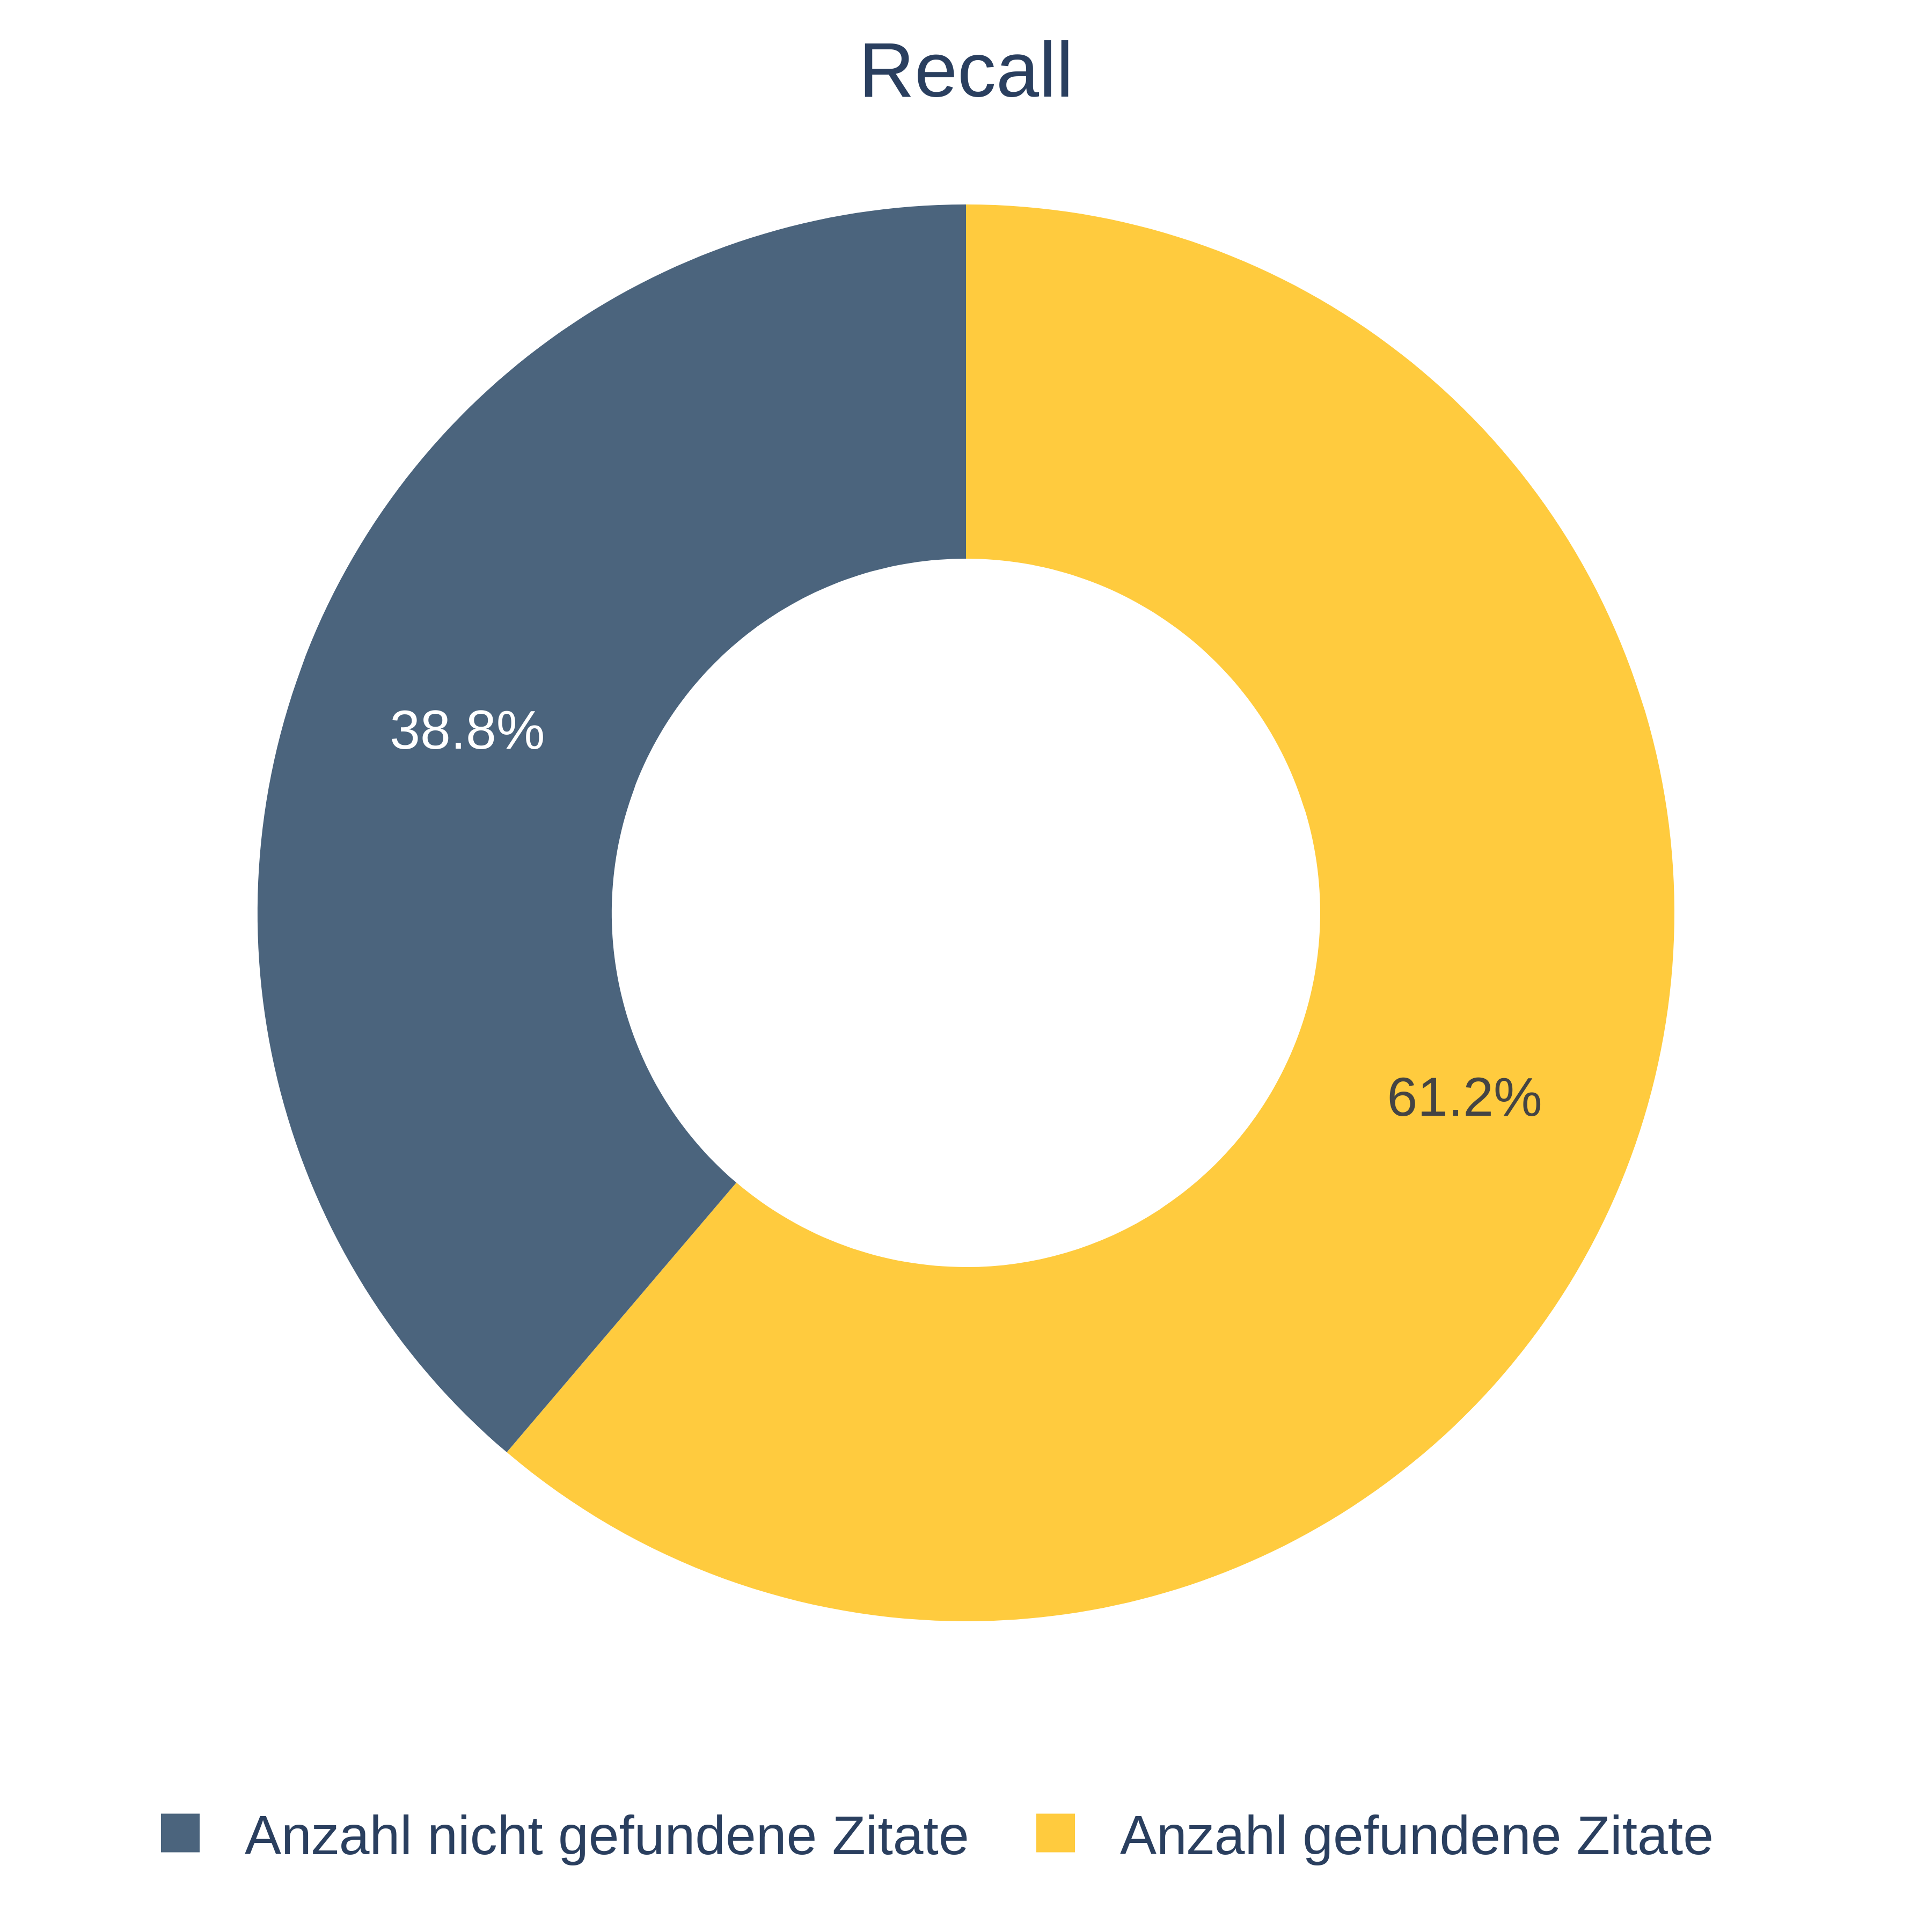
\includegraphics[width=0.75\linewidth]{./images/recall.png}
	\end{center}
	\caption{Recall der Zitate auf dem Testset}
	\label{piechart-recall}
\end{figure}

Das untenstehende Balkendiagramm \ref{barchart-recall} bietet einen Überblick
über die Performance aufgeschlüsselt nach Nachrichtenportal. Es fällt auf, dass
die Daten von Blick mit 70.6\% deutlich besser analysiert werden konnten als diejenigen
von 20min mit 50.0\%.

Wahrscheinlich ist diese Diskrepanz auf die geringe Anzahl Testfälle zurückzuführen.
Mit mehr Testfällen würde sich der Wert wahrscheinlich bei allen Nachrichtenportalen bei
60\% einpendeln.

\begin{figure}[H]
	\begin{center}
        \centering
		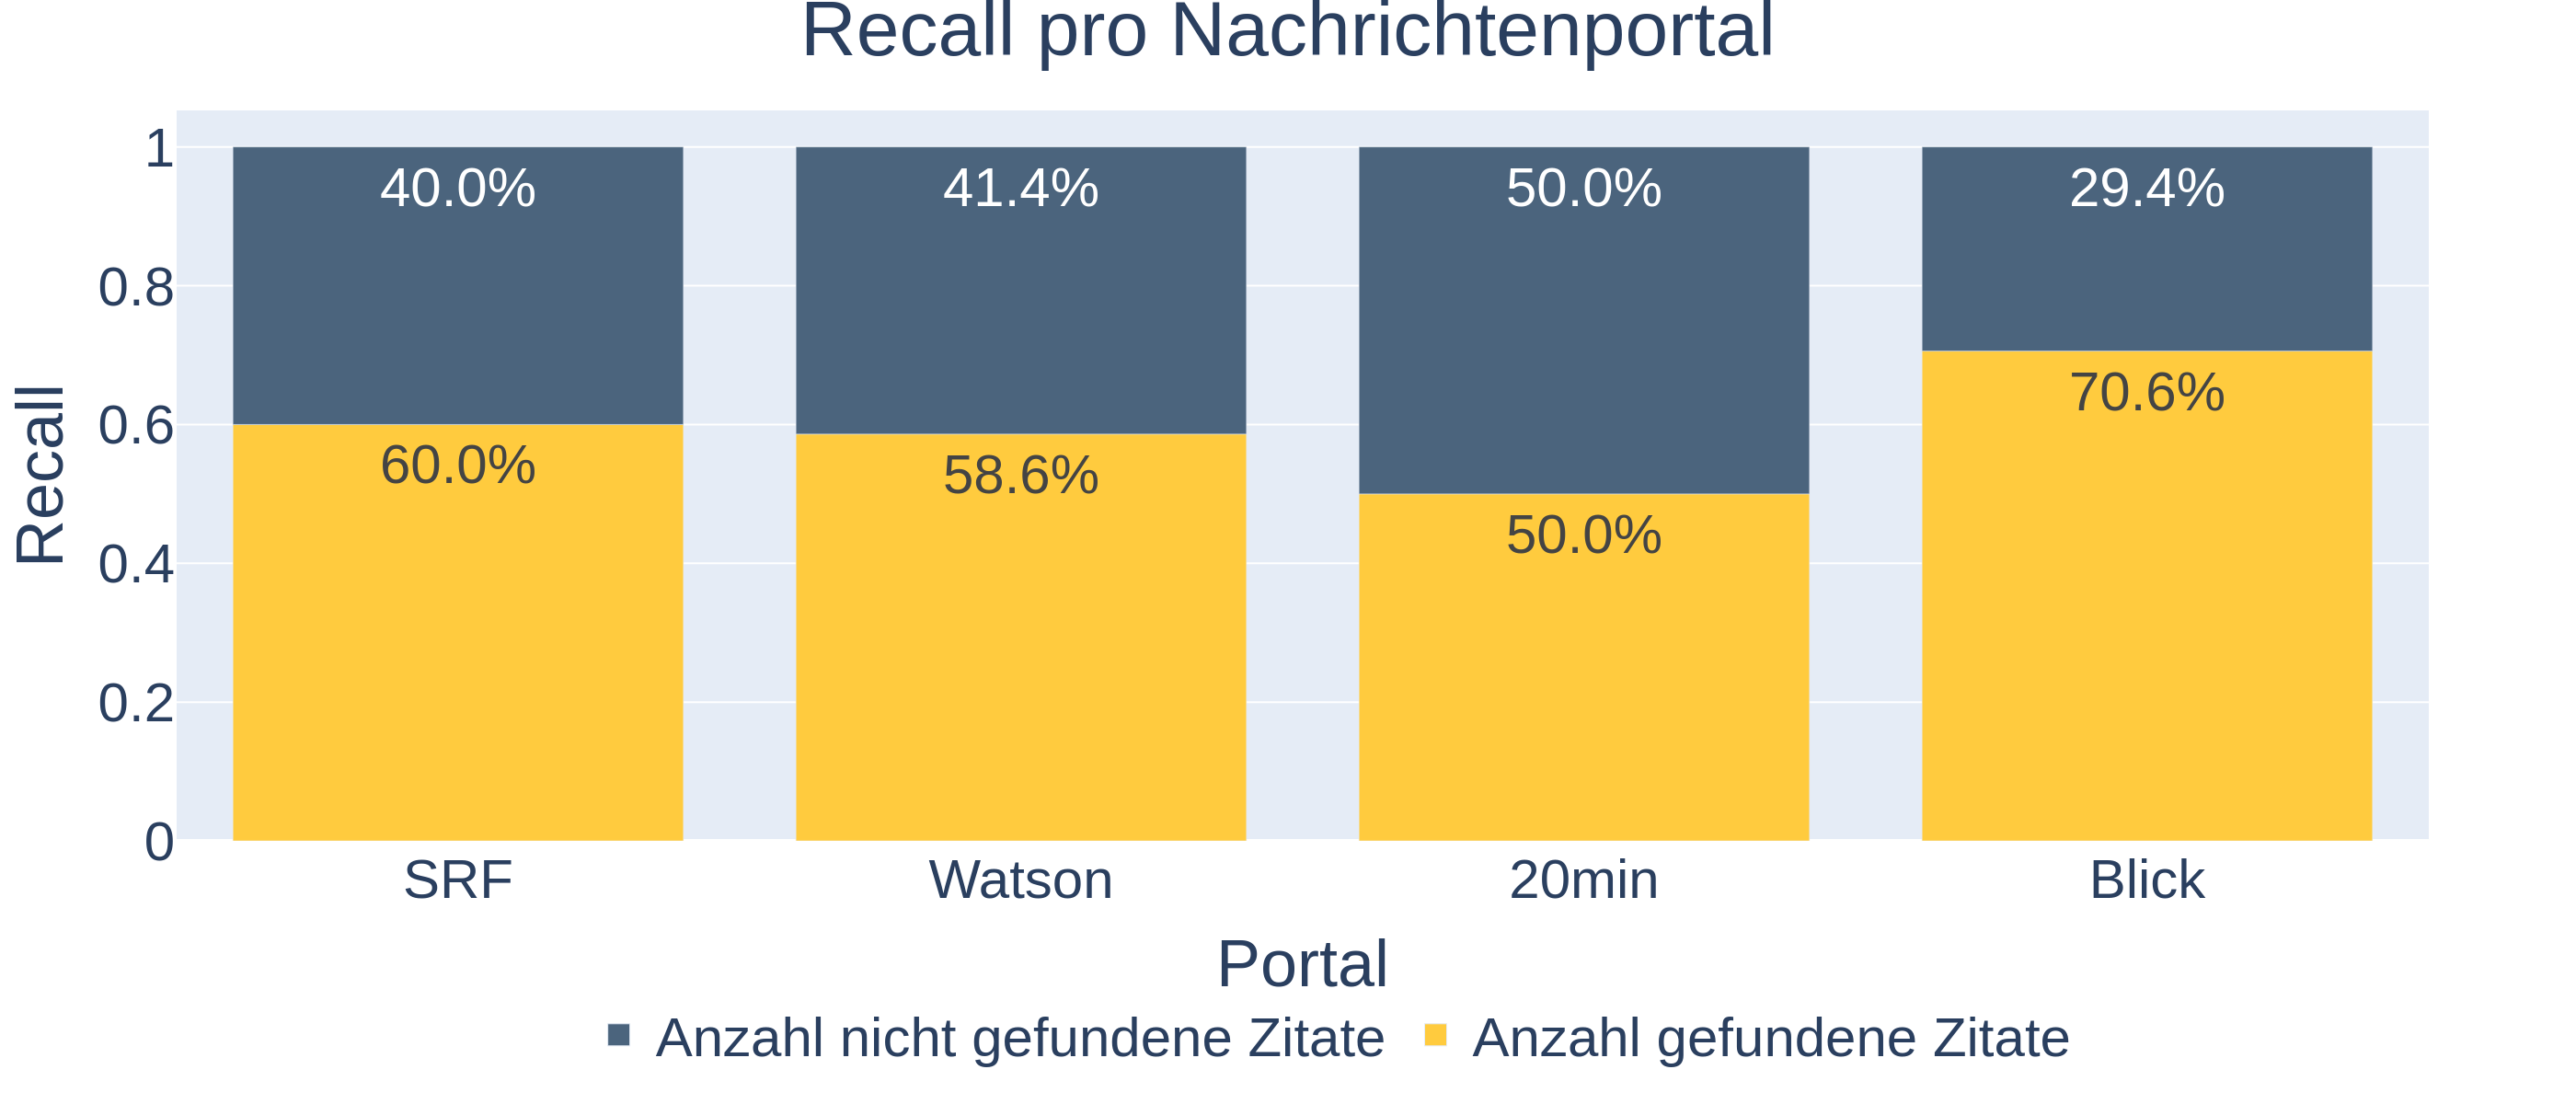
\includegraphics[width=1.0\linewidth]{./images/recall_portals.png}
	\end{center}
	\caption{Recall der Zitate pro Nachrichtenportal}
	\label{barchart-recall}
\end{figure}

\subsection{Qualitätsnote}\label{quality-grade}

Die Qualitätsnote setzt sich aus dem Durchschnitt der Stringähnlichkeiten der extrahierten Zitate
mit der Lösung zusammen. Zum Bestimmen der Stringähnlichkeit verwendet der Algorithmus den
\enquote{SequenceMatcher}\footnote{https://docs.python.org/3/library/difflib.html\#difflib.SequenceMatcher} von Python.
Dieser findet den länsten übereinstimmenden Substring aus zwei Strings relativ zur
Länge der beiden zu vergleichenden Strings.

Die Vermutung, dass die geringe Anzahl Tests Schwankungen in der Qualität verursacht
wird durch den Überblick in den folgenden Diagrammen (vgl. Abbildung \ref{histogram-grades}) gestützt.
20min hat deutlich weniger Zitate in den Lösungen als die anderen Nachrichtenportale.

Die Histogramme legen ausserdem nahe, dass die Rate der False-Positives gering ist.
Denn diese machen sich durch eine tiefe Note bemerkbar, da sie sehr unähnlich zu den Zitaten
aus den Lösungen sind. Dass davon wenige zu erkennen sind, suggeriert, dass False Positives
selten sind.

\begin{figure}[H]
	\begin{tabular}{ll}
		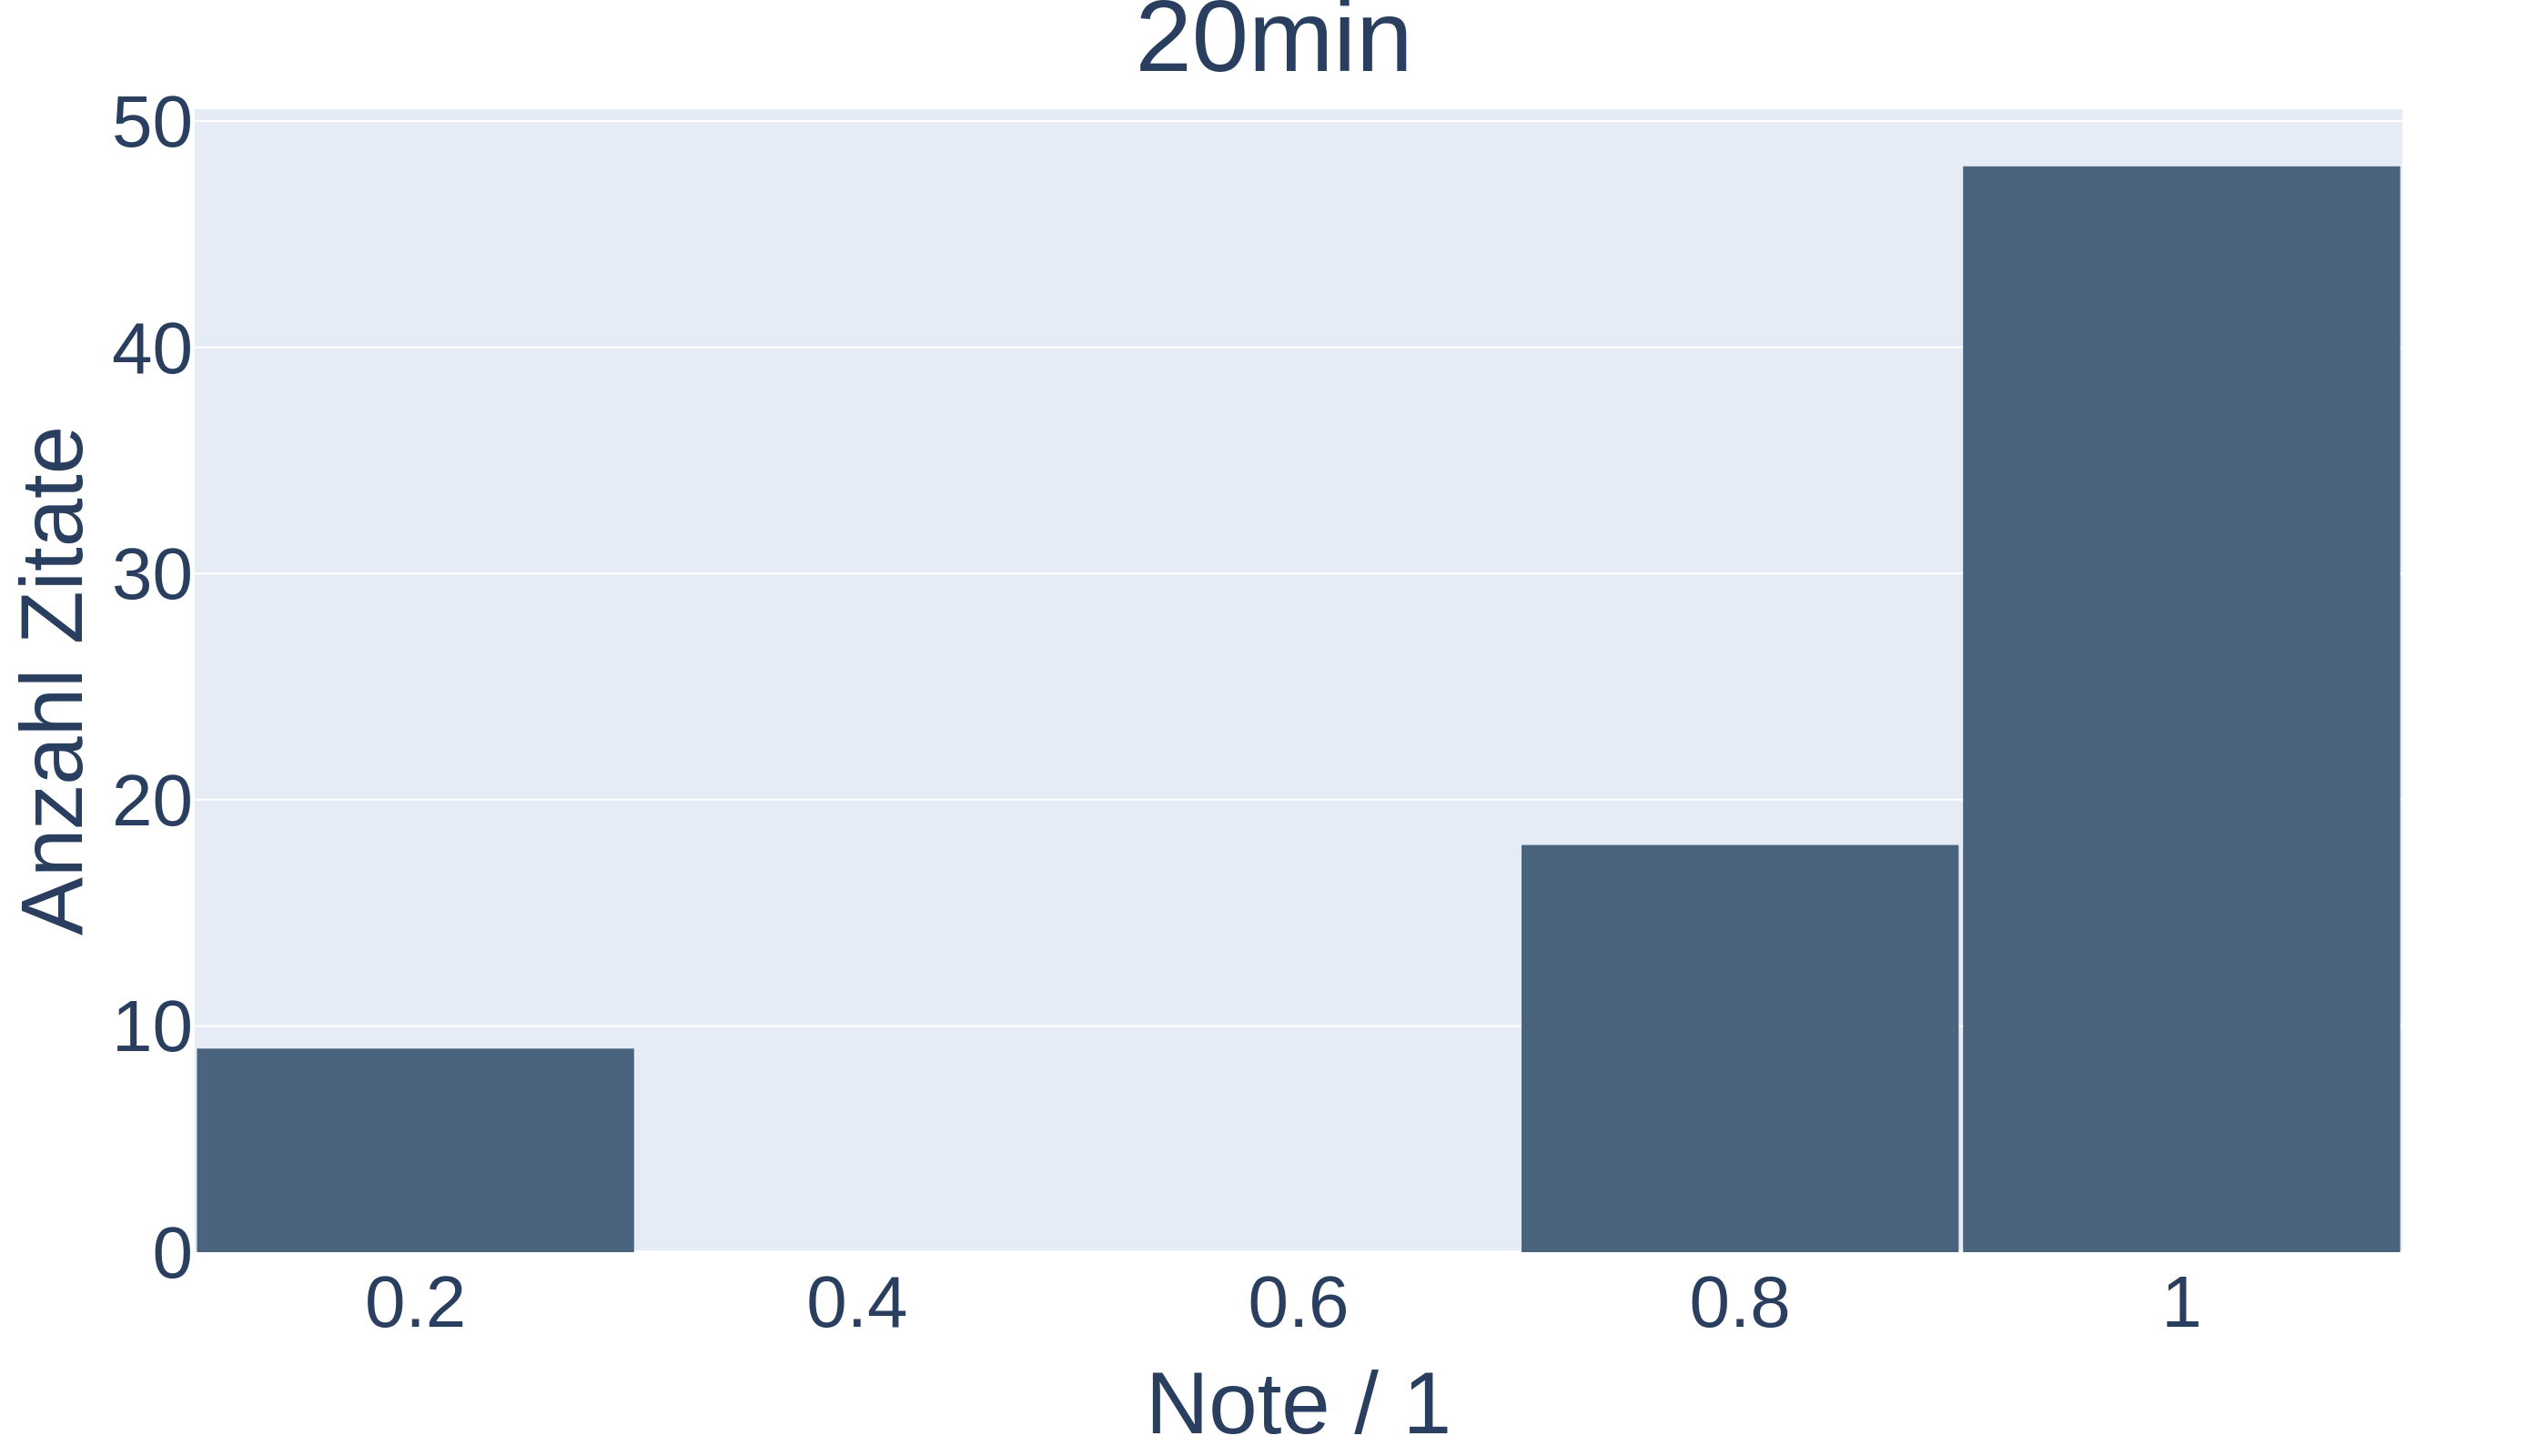
\includegraphics[width=.5\linewidth]{./images/citation_grades_20min.png} & 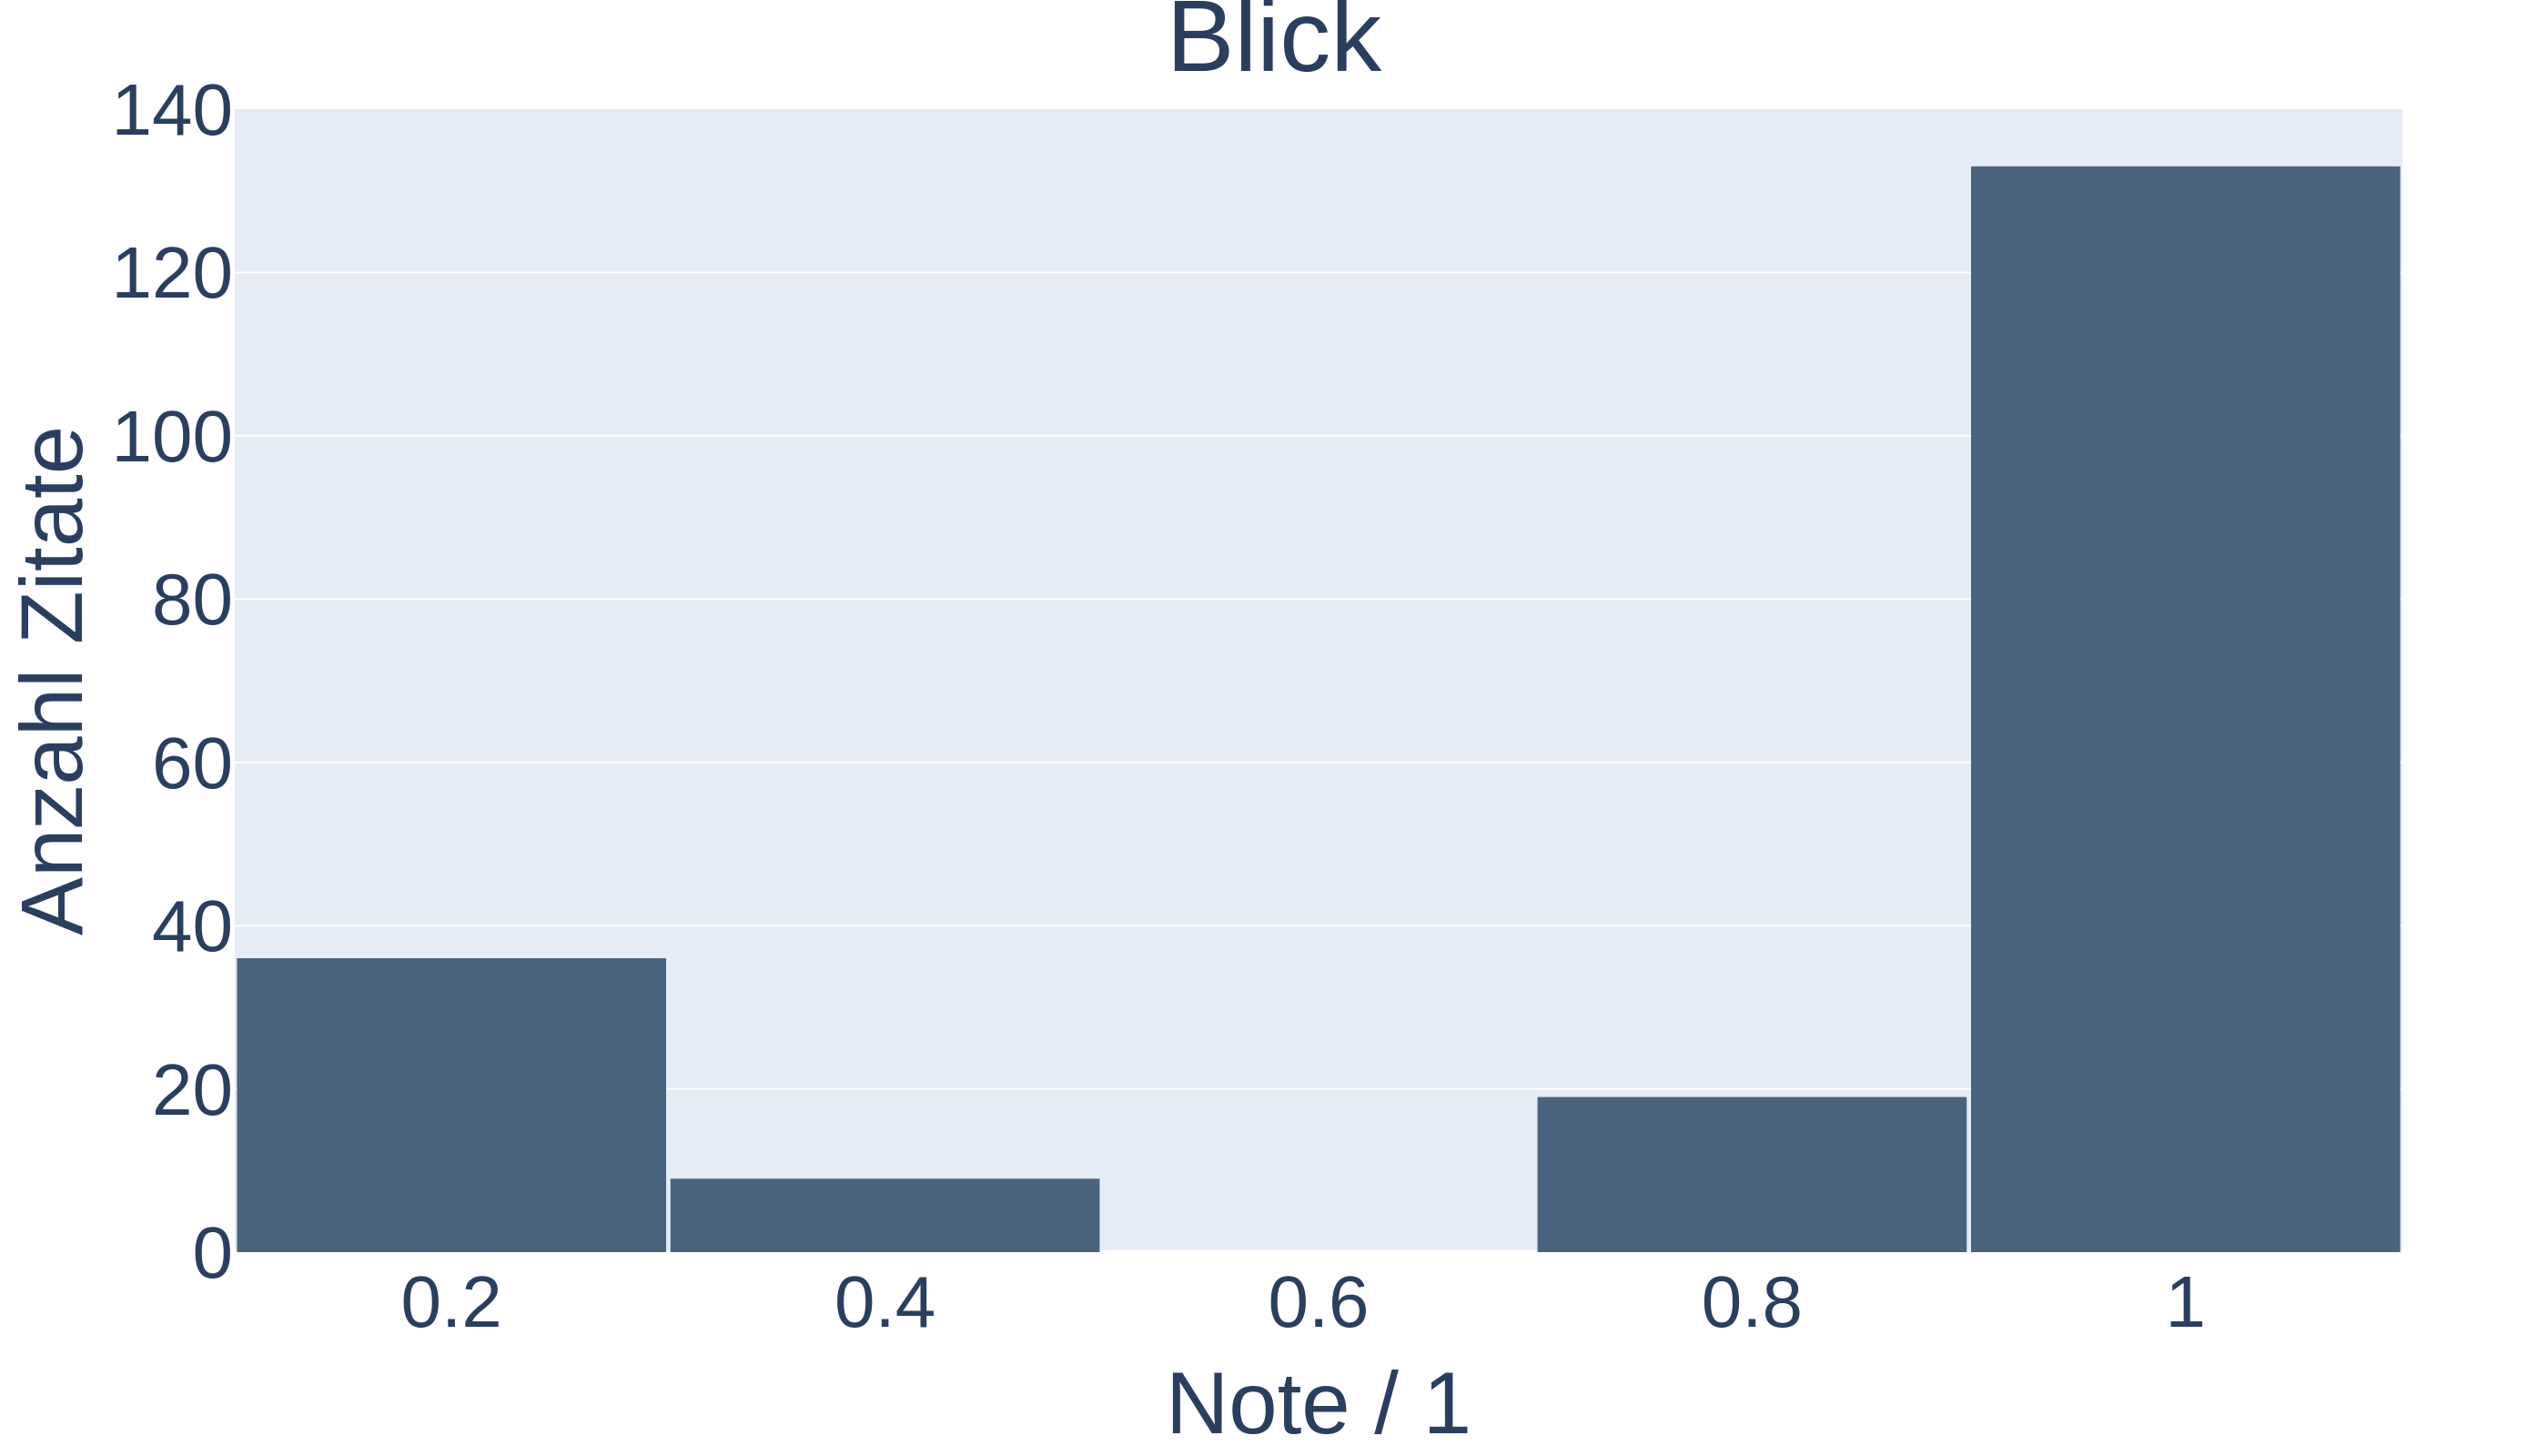
\includegraphics[width=.5\linewidth]{./images/citation_grades_blick.png} \\
		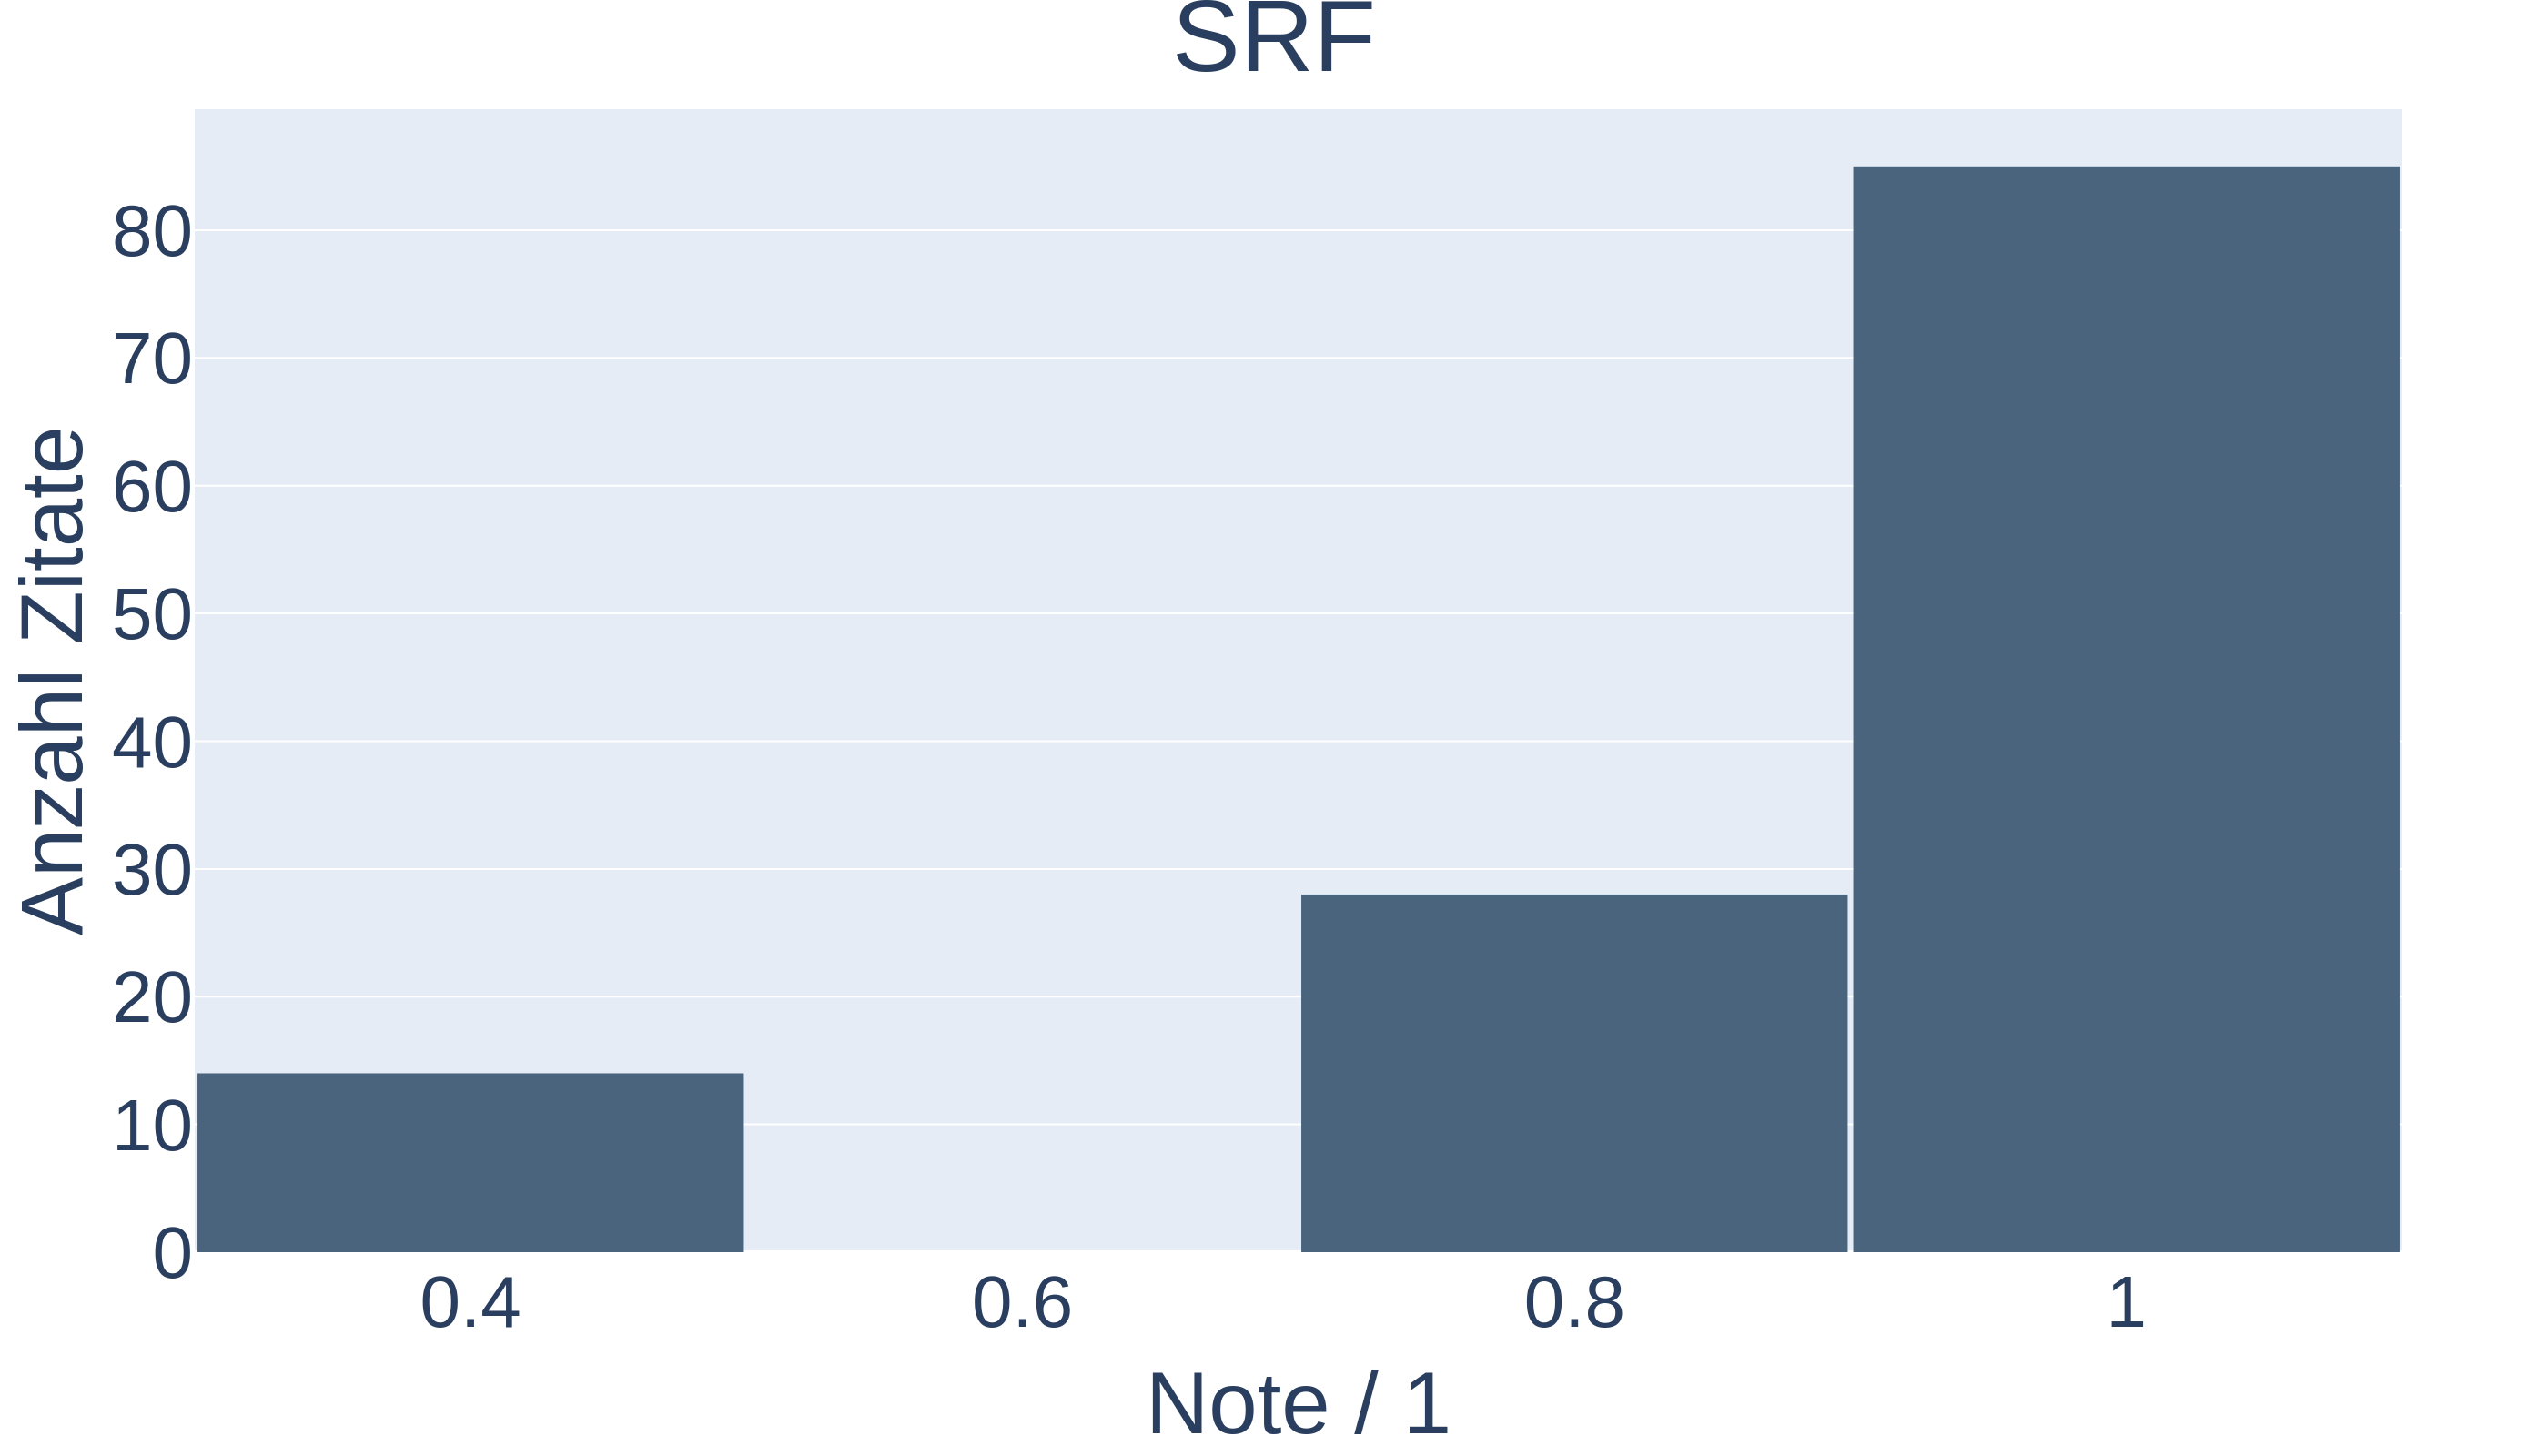
\includegraphics[width=.5\linewidth]{./images/citation_grades_srf.png} & 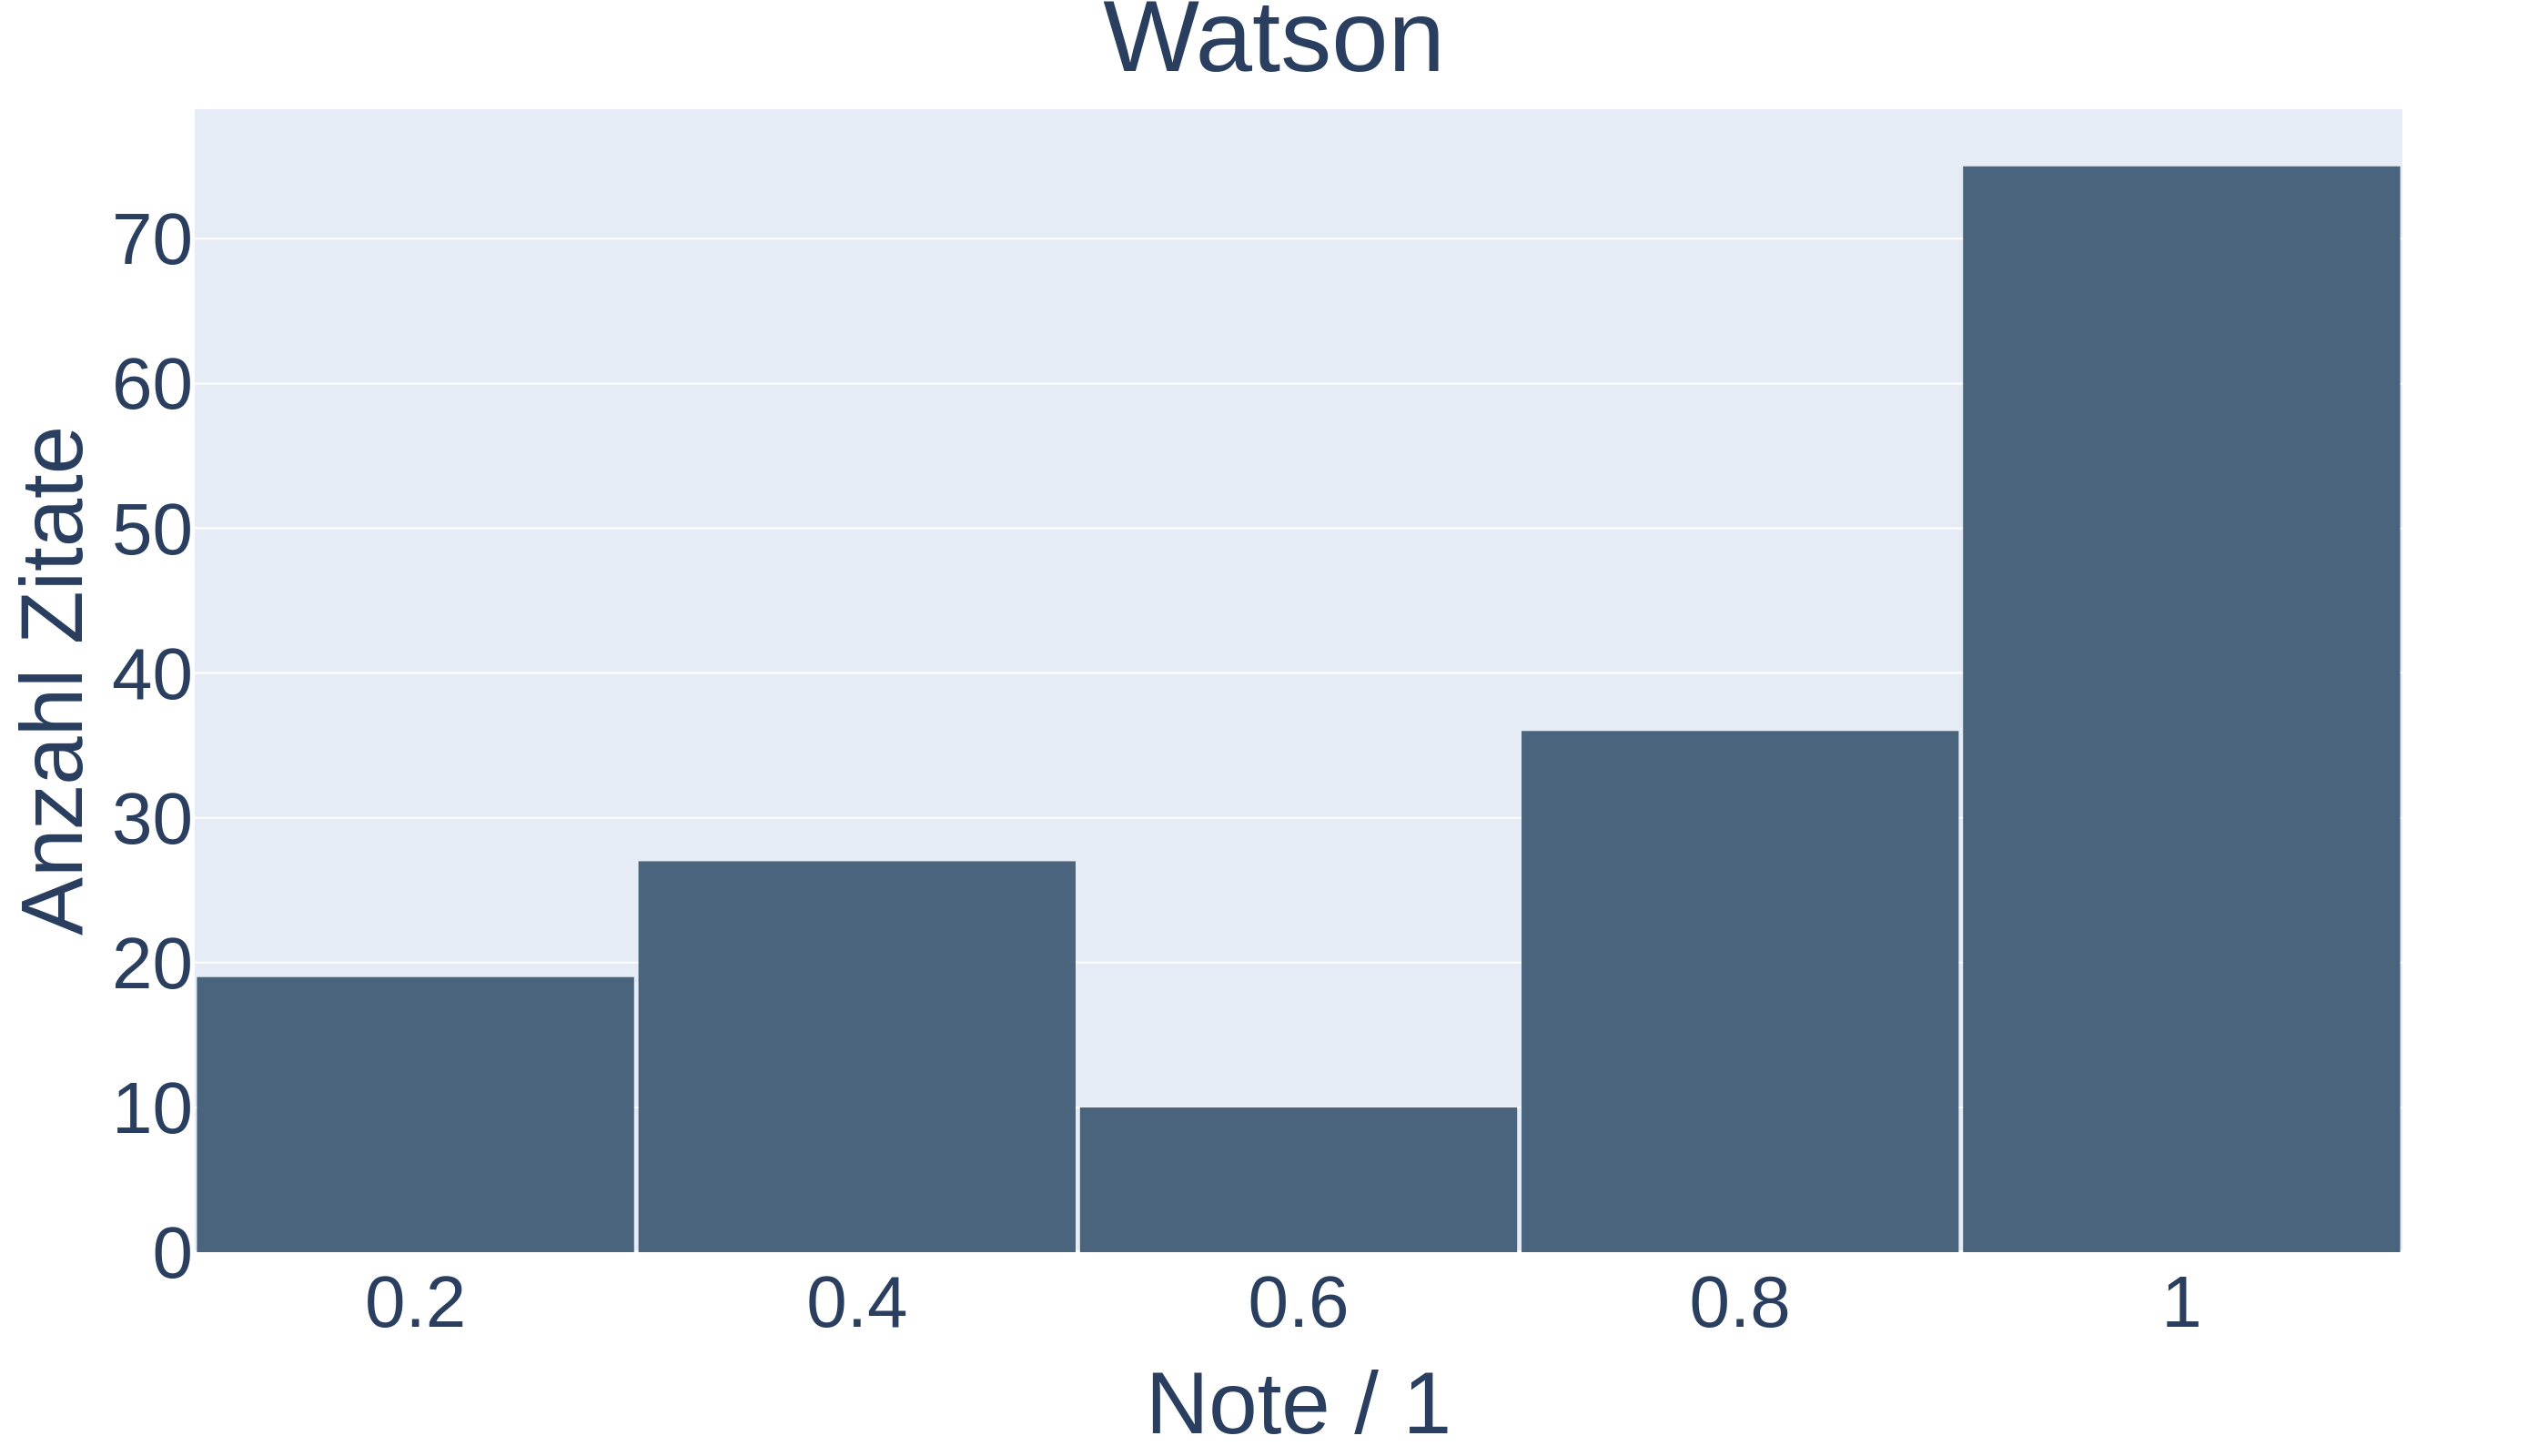
\includegraphics[width=.5\linewidth]{./images/citation_grades_watson.png} \\
	\end{tabular}
	\caption{Histogramme zur Verteilung der Qualität der gefundenen Zitate}
	\label{histogram-grades}
\end{figure}

\subsection{Nicht erkannte Zitate}\label{not-recognized-quotes}

Das nachfolgende Unterkapitel soll einen Überblick über die nicht erkannten Zitate liefern
und erklären, weshalb der Algorithmus aktuell noch nicht in der Lage ist, diese zu erkennen.

Grundsätzlich gibt es viele mögliche Erklärungen, weshalb das Programm gewisse Zitate nicht
erkennen kann. Aufgrund der analysierten Fälle scheinen die meisten fehlenden Zitate
entweder neuen, nicht implementierten Satzstrukturen oder Fehlern des Parsers geschuldet zu sein.

Es hat sich gezeigt, dass der Parser in langen Sätzen mit mehr als zwei Satzteilen
die Abhängigkeiten anders aufbaut. Deshalb wird der Subtree vom Algorithmus ignoriert.
So wird das Zitat einleitende Verb \enquote{schreibt} im folgenden Beispielsatz
als \enquote{mnr} (postnominal modifier) gekenntzeichnet (vgl. Abbildung \ref{citation-with-different-tree-structure-1}).
Wann und wie die gesuchten Verben mit diesem Label auftreten, konnten wir
nicht herausfinden.

\enquote{Dort habe er in einer Wohnung auch einen Grossteil seiner Sachen, unter anderem Familienerbstücke, wie das Inventar aus dem Restaurant Rossberg, wie der «Landbote» schreibt.}

\begin{figure}[H]
	\begin{center}
        \centering
		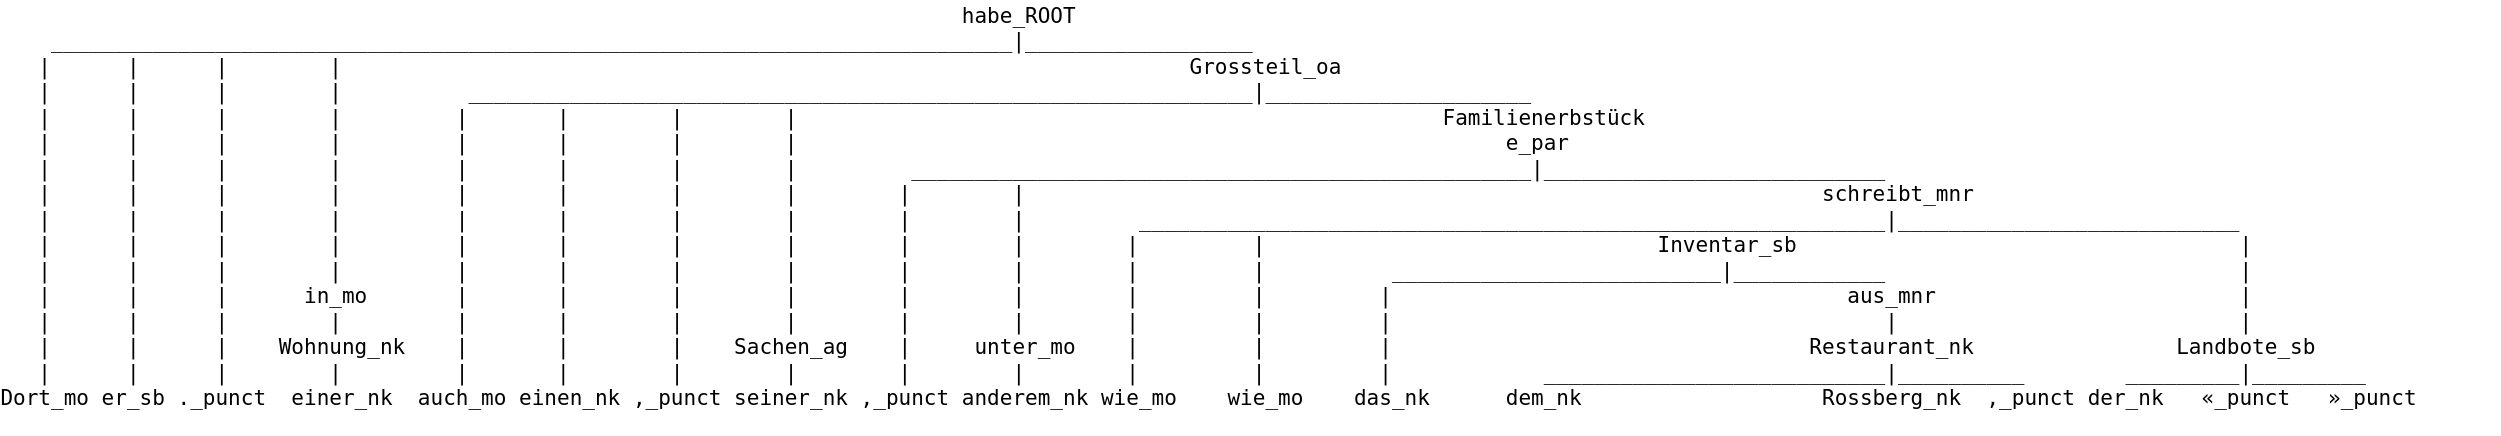
\includegraphics[width=1.0\linewidth]{./images/parse-tree-landbote.png}
	\end{center}
	\caption{Zitat mit anderer Baumstruktur}
	\label{citation-with-different-tree-structure-1}
\end{figure}

Bei dem nachfolgenden Satz wird das signifikante Verb \enquote{mitteilte} als \enquote{mo}
(modifier) gelabelt (vgl. Abbildung \ref{citation-with-different-tree-structure-2}).
In diesem Fall scheint der Parser das Label falsch vergeben zu haben,
denn \enquote{modifier}s werden meist den Adverben und Präpositionen zugeordnet.
Möglicherweise hat der Wortteil \enquote{mit} in diesem Fall den Ausschlag gegeben.

\enquote{Das Departement für Verteidigung, Bevölkerungsschutz und Sport (VBS) wird bis Ende Jahr die rechtlichen Grundlagen erarbeiten, wie der Bundesrat am Mittwoch mitteilte.}

\begin{figure}[H]
	\begin{center}
        \centering
		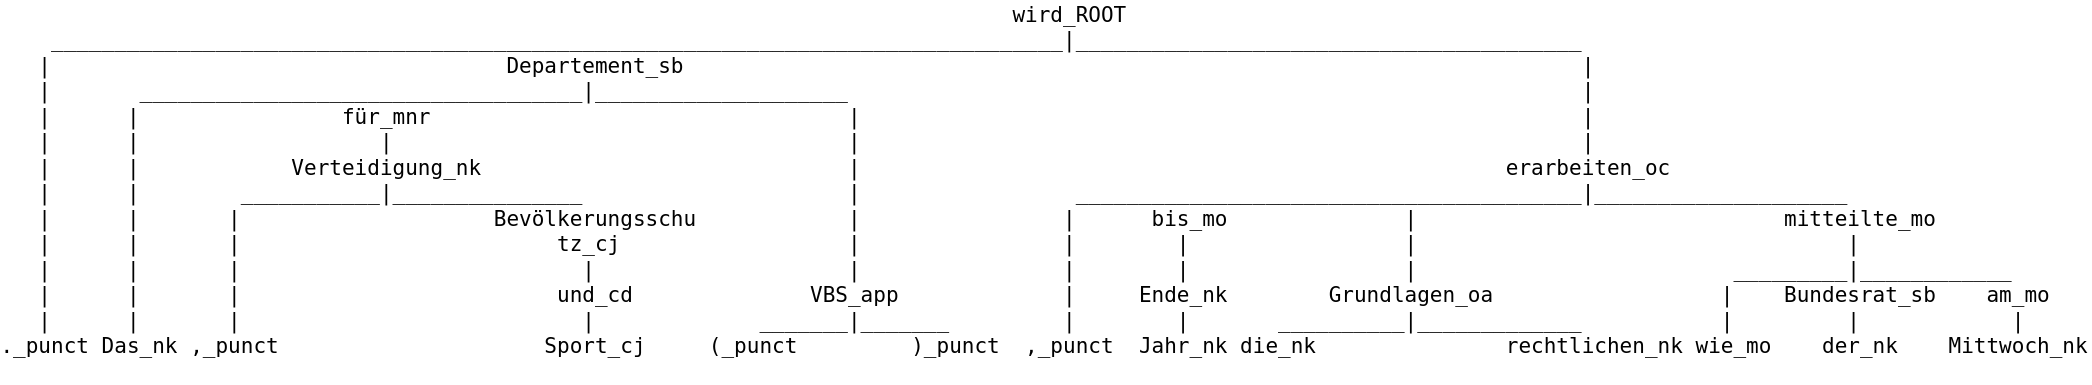
\includegraphics[width=1.0\linewidth]{./images/parse-tree-watson.png}
	\end{center}
	\caption{Zitat mit anderer Baumstruktur}
	\label{citation-with-different-tree-structure-2}
\end{figure}